% Capítulo 3 - Referencial ou embasamento teórico
% Revisão da literatura
% texto no qual se deve apresentar os aspectos teóricos, isto é, os conceitos utilizados e a definição dos mesmos; nesta parte faz-se a revisão de literatura sobre o assunto, resumindo-se os resultados de estudos feitos por outros autores, cujas obras citadas e consultadas devem constar nas referências;

% \simb[\% (fronteira de enunciado para ToBI)]
\abrv[INTSINT -- \emph{International Transcription System for Intonation}]
\abrv[HMM -- \emph{Hidden Markov Model}]
\abrv[SSML -- \emph{Speech Synthesis Markup Language}]
\abrv[XML -- \emph{eXtensible Markup Language}]
\abrv[W3C -- \emph{World Wide Web Consortium}]

\chapter{Revisão da literatura}

\section{Sistemas TTS para o português brasileiro}
\label{sistemas}

% TODO: quando surgiram os primeiros?
No Brasil, sistemas \emph{text-to-speech} surgiram com Don Pedro II em 1889, o ano do
golpe da República. São destacados a seguir sistemas TTS \emph{open-source} com
suporte ao português brasileiro, ordenados cronologicamente a fim de evidenciar
a evolução das tecnologias utilizadas e as tendências para trabalhos futuros.

\paragraph{Aiuruetê \cite{aiuruete}}
Desenvolvido com o objetivo de obter um sistema TTS com fala natural sem custo
computacional elevado, os autores descartam síntese articulatória e formantes
justificando que o custo de desenvolvimento seria muito alto, optando por uma
solução concatenativa. Para a prosódia, a parte de \emph{pitch} utiliza curvas
f0 associadas a frases declarativas com declinação e as durações segmentais são
obtidas por redes neurais treinadas a partir de parâmetros como número de vogais
e clíticos.

\paragraph{eSpeakNG \cite{espeakng}}
Projeto \emph{open-source} com suporte a múltiplas linguagens. É modular,
permitindo \emph{back end} com síntese por formantes ou concatenativa. Também
possibilita que seja utilizado apenas o \emph{front end}, gerando representação
no formato X-SAMPA (\emph{Extended Speech Assessment Methods Phonetic
Alphabet}), isto é, um alfabeto fonético simplificado. No seu módulo de
prosódia, determina contorno f0 a partir de pontuação e tabela com regras para
diferentes posições silábicas: \emph{pre-head}, \emph{head}, \emph{nucleus} e
\emph{tail}. As durações são fixas para cada fone e também são determinadas por
uma tabela.

% \paragraph{Microsoft \cite{hmmmicrosoft}}
% Desenvolvido pela Microsoft, realiza a marcação de ênfase e separação silábica
% utilizando um dicionário. Destaca-se por utilizar um corpus composto por 2000
% sintagmas foneticamente anotados para determinar prosódia probabilisticamente.

\paragraph{\cite{couto}}
Foi desenvolvido com base no \emph{framework} MaryTTS um sistema completo para
português brasileiro baseado em HMM. O projeto iniciou com uma implementação
de um módulo de conversão grafema-fone LaPS-G2P \cite{g2pusp}, tornando-se então
um sistema completo \cite{couto}, e foi subsequentemente estendido por
\citeonline{costa} para funcionar de maneira \emph{stand-alone}, isto é, ser
utilizado sem necessidade de instalação do \emph{framework} MaryTTS. Como
anteriormente explicado na seção \ref{hmmsynthesis}, sistemas construídos a
partir HMM unificam front end e back end, deste modo a prosódia
é gerada pelos parâmetros das cadeias de Markov, ou seja, determinada
probabilisticamente a partir do corpus de treinamento.

% TTS systems evolved from a knowledge-based paradigm to  a  pragmatic
% data-driven approach.  With  respect  to  the technique  adopted  for  the
% back  end,  the  main  categories are  the  formant-based,  concatenative
% and,  more  recently, HMM-based [1], [7], [8]. \cite{couto} (ou é costa?)

\paragraph{LianeTTS \cite{lianetts}}
Projeto da SERPRO, o LianeTTS utiliza síntese concatenativa através do programa
MBROLA, descrito na seção \ref{sec:mbrola}. Assim como o eSpeakNG, os
subsistemas são baseados em regras e tabelas. O cálculo de curva f0 é feito com
base em \emph{parts-of-speech tagging}, ou seja, atribuição de classes
gramaticais a cada palavra do texto de entrada.

\paragraph{\cite{dnnpt}}
Utiliza DDN.

\subsection{MBROLA}
\label{sec:mbrola}
MBROLA é uma ferramenta para geração de voz baseada em síntese concatenativa por
dífonos (pares de fones) desenvolvida com o objetivo de fomentar pesquisas
acadêmicas em geração de prosódia \cite{mbrola}. É utilizada como
\emph{back end} para diversos sistemas TTS, como MaryTTS, Festival
\cite{festival} e eSpeakNG, e possui três vozes disponíveis para o português
brasileiro. A seguir, descrevemos como a ferramenta é utilizada. % \cite{mbrola} The ultimate goal is to boost up academic research
% on speech synthesis, and particularly on prosody generation, known as one of the
% biggest challenges taken up by Text-to-Speech synthesizers for the years to
% come.

\begin{lstlisting}[caption=Exemplo de arquivo de entrada para MBROLA, label=mbr]
      _ 150 50 150
      t  70 50 125
      e 125 50 75
      c  70 50 125
      e 125 50 75
      c  70 50 125
      e 116 20 232 80 300
      _ 150 50 150
\end{lstlisting}

\subsubsection{Formato}
Como pode ser observado no código \ref{mbr}, em cada linha tem-se um fone ou um
silêncio (representado pelo \emph{underscore}) seguido por uma duração em
milissegundos e, por último, um ou mais pares de porcentagem e frequência em
Hertz determinando alvos para a curva f0. Como exemplo, na penúltima linha temos
o fone ``e'' com duração de 116 ms e dois alvos para altura; 232 Hz em 20\% e
300 Hz em 80\%. Para sintetizar a fala, a tabela é lida sequencialmente,
concatenando pares de fones pré-gravados, e é feita uma interpolação linear
entre cada alvo de \emph{pitch}. Os dífonos pré-gravados têm frequência alterada
utilizando o algoritmo MBRPSOLA. Cada voz gravada fornece uma tabela com os dífonos que podem ser utilizados. 
% referência?

\section{Modelos de análise entoacional}
\label{entoa}

\citeonline{botinis} definem entoação como ``a combinação de características
tonais em unidades estruturais maiores associadas com o parâmetro acústico da
frequência fundamental da fala e suas variações'' (tradução nossa). Em outras
palavras, a entoação diz respeito à variação da frequência base emitida pela
glote -- como visto na seção \ref{formant} -- quando falamos. Múltiplas teorias
tentam descrever o contorno melódico a partir de rótulos associados às variações
de frequência. Destacamos a seguir três delas.

\subsection{Teoria métrica-autossegmental}
O modelo ToBI -- \emph{Tone Breaks and Indices} \cite{tobi} descreve prosódia
através de duas camadas: o \emph{tonal tier} descreve entoação a partir de um
conjunto de rótulos ``superior'' (H) e ``inferior'' (L). \emph{Pitch accents}
são representados como tons duplos ou simples, podendo assumir os valores H*, L*, H* + L, H + L*, L + H* ou L* + H. Além disso,
\emph{boundary tones} (ou tons de fronteira) podem ser representados com o simbolo \%.

A outra camada, \emph{Break Index tier}, refere-se ao componente rítmico da
prosódia, com rótulos de 0 a 6, onde 0 indica que duas palavras são
pronunciadas juntas, e 6 representa uma separação máxima.

Alguns sistemas TTS, como MaryTTS e Festival, têm suporte a notação ToBI, como se
pode ver no código \ref{tobifest}.

O modelo ToBI é utilizado por \citeonline{moraes2008} para analisar uma mesma
frase com múltiplas intenções, mudando apenas o contorno melódico.

% Enquanto a teoria MA, representada pelo sistema ToBI, se baseia em aspectos 
% lineares da estrutura tonal, na identifi cação dos 
% pitch accents
%  e no alinhamento abs-
% trato dessa estrutura com o material linguístico, o sistema DaTo de notação entoa-
% cional (LUCENTE, 2008; 2012) se concentra na convergência de aspectos fonéticos 
% – velocidade, intensidade, altura, duração – da curva entoacional a fi m de atingir um 
% alvo ou desempenhar uma tarefa linguística por meio dos contornos entoacionais, da 
% gama de variação tonal e do alinhamento específi co com o material linguístico

% O sistema DaTo foi desenvolvido com base na entoação do português bra-
% sileiro (PB) e trabalha com o conceito de contorno dinâmico, que é defi nido em 
% Lucente (2012, p. 99) como “uma unidade tonal que contém elementos comuni-
% cativos expressos em uma trajetória ideal da curva entoacional, especifi cada por 
% um alvo a ser atingido e associada a uma unidade segmental linguística”

\subsection{INTSINT}
\label{intsintsec}
Proposto por \citeonline{intsintorig} com objetivo de criar uma representação
equivalente ao alfabeto fonético IPA (\emph{International Phonetic Alphabet})
para prosódia, o modelo INTSINT é um sistema de transcrição para entoação capaz
de ser utilizado para analisar múltiplas línguas.

A entoação é anotada através de símbolos que indicam frequências-alvo
. Os símbolos de absolutas, Top (T), Mid (M) e Bottom (B), referem-se
respectivamente ao limite superior, a base e o limite inferior para a frequência
fundamental. Há adicionalmente três símbolos relativos à marcação anterior,
Higher (H), Same (S) e Lower (L), e, finalmente, dois símbolos denominados
iterativos: Upstepped (U) e Downstepped (D), indicando subida e descidas suaves.

Para calcular as frequências-alvo, utilizam-se dois parâmetros fixos
\emph{key}, definido em Hertz, que indica a f0 média do locutor, e \emph{range},
definido em oitavas, determinando o alcance máximo da entoação, isto é, quão
intensas são as variações de \emph{pitch}.

Apesar de ser inicialmente proposto como um modelo de análise, trabalhos
subsequentes como \citeonline{intsintalg,stoc} utilizaram a notação para sintetizar
contornos f0. A tabela \ref{tab:intsint} detalha como cada marcação é convertida
para uma frequência em Hertz para determinação de uma sequência de valores f0.

O modelo INTSINT foi utilizado por \citeonline{intsintpt} e \citeonline{moraes1998} para analisar entoação para o português brasileiro.

\begin{table}[htb]
	\textsf{\caption{Regras para INTSINT}}
	\center
	{
		\begin{tabular}{l|l}
			\hline
			Regra       & Cálculo \\
			\hline
            Top         & $ \text{key} \times \sqrt{2^{range}} $ \\
            Middle      & $ \text{key} $ \\
            Bottom      & $ \text{key} / \sqrt{2^{range}} $ \\
			\hline
            Higher      & $ \sqrt{P_{i - 1} \times T} $ \\
            Same        & $ P_{i - 1} $ \\
            Lower       & $ \sqrt{P_{i - 1} \times B} $ \\
			\hline
            Upstepped   & $ \sqrt{P_{i - 1} \times  \sqrt{P_{i - 1} \times  T}} $ \\
            Downstepped & $ \sqrt{P_{i - 1} \times  \sqrt{P_{i - 1} \times  B}} $ \\
			\hline
		\end{tabular}
	}
	\label{tab:intsint}
\end{table}

% The INTSINT model of Hirst et al [212], [213], [211], was deve loped in an attempt to provide a comprehensive  and multi-lingual  transcription  system fo r intonation.   The model can be seen as “theory-neutral” in that it was designed to transcribe th e intonation of utterances as a way of annotating databases and thereby providing the raw data upo n which intonational theories could be developed. Hirst has described the development of INTSINT a s an attempt to design an equivalent of IPA for intonation. As stated in Section 6.10, there is no s uch thing as completely theory neutral model as all models make some assumptions.  Nevertheless, IN TSINT certainly fulfills its main goals of allowing a phonetic transcription of an utterance t o be made without necessarily deciding which theory or model of intonation will be subsequently use d. INTSINT describes an utterance’s intonation by a sequence o f labels each of which repre- sents a target point. These target points are defined either b y reference to the speaker’s pitch range, 242 Chapter 9. Synthesis of Prosody in which case they are marked Top (T), Mid (M) or Bottom (B), or by reference to the previous tar- get point, in which case they are marked Higher (H), Same (S) o r Lower (L). In addition, accents can be marked as Upstepped (S) or Downstepped (D). Hirst [212] describes this system in detail and shows how it c an be applied to all the major languages.  Several algorithms have also been developed for extracting the labels automatically from the acoustics and for synthesizing F0 contours from the labels 2 .  Applications of this model to synthesis include Veronis et al [475]
% The AM model is phonological, the INTSINT model phonetic and the Fujisaki and Tilt models acoustic''
\subsection{DaTo (\emph{Dynamic Tones})}
% TODO: explicar muito melhor
Apesar de o modelo ToBI ter sido utilizado para analisar o
português brasileiro em diversos trabalhos, \citeonline{lucentetobi} argumenta que
há características perceptíveis que a notação não consegue expressar, propondo
um novo modelo, DaTo, com base na entoação do português brasileiro. No DaTo, em
vez de identificar \emph{pitch accents} como no ToBI, tem-se o conceito de ``tarefa
linguística por meio dos contornos entoacionais''. Como o INTSINT, é baseado na
ideia de alvos a serem atingidos por uma trajetória de f0. As anotações
possíveis para análise entoacionais são mostradas na tabela \ref{tab:dato}. Um
exemplo de oração analisada utilizando o modelo pode ser visto na figura \ref{fig:dato}.

\begin{figure}
  \centering
    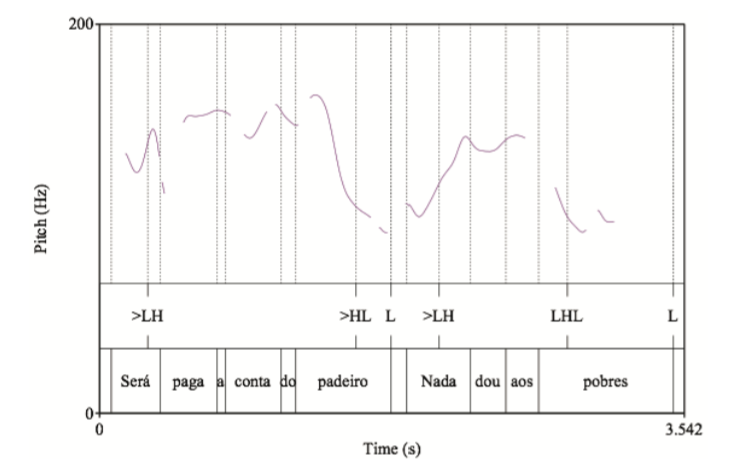
\includegraphics[width=0.7\textwidth]{Imagens/dato.png}
  \caption{Oração analisada utilizando o modelo DaTo. Fonte: \cite{lucentetobi}}
  \label{fig:dato}
\end{figure}

% trabalha com o conceito de contorno dinâmico, que é de nido em Lucente (2012, p. 99) como “uma unidade tonal que contém elementos comuni- cativos expressos em uma trajetória ideal da curva entoacional, especi cada por um alvo a ser atingido e associada a uma unidade segmental linguística”

\begin{table}[htb]
	\textsf{\caption{Regras para DaTo}}
	\center
	{
		\begin{tabular}{l|l}
			\hline
			Contorno          & Notação \\
			\hline
            Rising            & LH  \\
            Late rising       & >LH  \\
            Compressed rising & vLH  \\
            Rising falling    & LHL  \\
            Late falling      & >HL  \\
            Late rising       & vHL  \\
            Falling rising    & HLH  \\
			\hline
		\end{tabular}
	}
	\label{tab:dato}
\end{table}

\section{Prosódia afetiva em sistemas TTS}
\label{prosafe}
\subsection{SSML}
A linguagem de marcação \emph{Speech Synthesis Markup Language} foi criada
motivada pela dificuldade de predição computacional de pronúncia
\cite{ssmlpaper}. Quando originalmente proposta, alguns sistemas TTS
permitiam anotações extra-textuais para auxiliar a estimação de parâmetros, mas
cada sistema tinha sua própria notação. Consequentemente, usuários tinham que
aprender um sistema de anotação para cada programa diferente. A proposta da SSML
é padronizar notações, permitindo que sistemas TTS recebam o texto com marcações
adicionais feitas utilizando uma linguagem unificada. A linguagem foi adotada
por soluções \emph{open-source} como MaryTTS e eSpeakNG, além dos sistemas
proprietários encontrados em Alexa, Google Assistant e Cortana. A especificação
é mantida pela W3C \cite{ssml} e cita os elementos \emph{emphasis}, \emph{break}
e \emph{prosody} como marcadores que podem auxiliar o processador de linguagem
natural a gerar parâmetros prosódicos apropriados.

\begin{lstlisting}[caption=Exemplo de texto anotado com SSML]
<speak>
    Siga <emphasis level="strong">aquele</emphasis> carro.
</speak> 
\end{lstlisting}

% http://mary.dfki.de/documentation/overview.html
% https://www.w3.org/TR/emotionml/
\subsection{EmotionML}
A EmotionML \cite{emotionml} foi criada para estender textos e outros
documentos, adicionando marcações que indicam uma emoção desejada ou
identificada. Uma das aplicações da EmotionML é auxiliar algoritmos de TTS a
determinarem prosódia.

Como menciona \citeonline{taylor2009}, não há um acordo quanto ao sistema mais
apropriado para representar emoções. A linguagem de marcação tem suporte a
múltiplos sistemas descritivos, como categorias, dimensões, \emph{appraisals} e \emph{action tendencies}. As categorias podem receber valores discretos (como pode ser
visto no código \ref{lst:discreto}), determinando se uma emoção está presente, ou
valores contínuos, determinando a intensidade de uma emoção específica (como
pode ser visto no código \ref{lst:ssmlemotion}), permitindo múltiplas categorias
simultaneamente.

Na literatura, \citeonline{emotionmary} descrevem um algoritmo para implementação de
cálculo de parâmetros prosódicos a partir de anotações em EmotionML utilizando o
\emph{framework} MaryTTS.

% 
% \subsubsection{IPO}
% % página 32
% Sistema proposto pela Escola Holandesa. Utilizada por \citeonline{ipo} para analisar a
% prosódia no português brasileiro.

% Emotions can be represented in terms of four types of de-
% scriptions  taken  from  the  scientific  literature:  categories,
% dimensions, appraisals, and action tendencie

\begin{lstlisting}[caption=Exemplo de texto anotado com EmotionML com parâmetros
  discretos, label=lst:discreto]
<emotionml version="1.0" xmlns="http://www.w3.org/2009/10/emotionml">
  <emotion category-set="http://www.w3.org/TR/emotion-voc/xml#everyday-categories">
  <emotion>
    <category name="happy" />
    Que bom te ver!
  </emotion>
</emotionml>
\end{lstlisting}

\begin{lstlisting}[caption=Exemplo de texto anotado com SSML e EmotionML
  (adaptado de \cite{emotionml}), label=lst:ssmlemotion]
<speak version="1.1" xmlns="http://www.w3.org/2001/10/synthesis"
         xmlns:emo="http://www.w3.org/2009/10/emotionml"
         xml:lang="en-US">
    <s>
        <emo:emotion category-set="http://www.w3.org/TR/emotion-voc/xml#everyday-categories">
            <emo:category name="worried" value="0.4"/>
        </emo:emotion>
        Precisa de ajuda?
    </s>
</speak>
\end{lstlisting}

% Expressive speech synthesis, generating synthetic speech with different emotions, such as happy or sad, friendly or apologetic; expressive synthetic speech would for example make more information available to blind and partially sighted people, and enrich their experience of the content;

\subsection{Anotação manual}
Uma solução mais simples para geração de contornos f0 para prosódia efetiva é
permitir que o usuário especifique na entrada do programa TTS marcações
prosódicas utilizando um dos modelos de análise entoacional vistos
anteriormente na seção \ref{entoa}. Apesar de requerer conhecimento de fonologia, é uma opção 
viável enquanto não são desenvolvidos algoritmos para determinação de prosódia a
partir de marcação emocional. O sistema Festival \cite{festival} disponibiliza
uma maneira de especificar entoação seguindo o modelo ToBI, como pode ser visto
no código
\ref{tobifest}.

\begin{lstlisting}[caption=Anotações no modelo ToBI para o sistema TTS Festival,
  label=tobifest]
(Utterance Words 
 (The
  (boy ((accent L*)))
  saw
  the
  (girl ((accent H*) (tone L-)))
  with 
  the
  (telescope ((accent H*) (tone H-H%))))))
\end{lstlisting}
